\documentclass[fontsize=9pt]{scrartcl}
\usepackage[inline]{asymptote}

\usepackage{amsmath, amssymb}
\usepackage{mlmodern}
\usepackage[most]{tcolorbox}
\usepackage{tikz}
\usepackage{asymptote}
\usepackage[a4paper, total={6.5in, 10.25in}]{geometry}
\begin{document}
	\title{ Problems: }
	\author{}
	\date{}
	\maketitle
	\begin{tcolorbox}
		[colback=white!5!white,colframe=purple!75!white,title=\textsf{Problem 1: (USA
		EGMO Team Selection Test 2020)}, opacityback=1] Vulcan and Neptune play a turn-based
		game on an infinite grid of unit squares. Before the game starts, Neptune chooses
		a finite number of cells to be flooded. Vulcan is building a levee, which is
		a subset of unit edges of the grid (called walls) forming a connected, non-self-intersecting
		path or loop*.

		The game then begins with Vulcan moving first. On each of Vulcan’s turns, he
		may add up to three new walls to the levee (maintaining the conditions for
		the levee). On each of Neptune’s turns, every cell which is adjacent to an already
		flooded cell and with no wall between them becomes flooded as well. Prove
		that Vulcan can always, in a finite number of turns, build the levee into a
		closed loop such that all flooded cells are contained in the interior of the
		loop, regardless of which cells Neptune initially floods. ~\\ ~\\ \emph{ *More
		formally, there must exist lattice points $\mbox{\footnotesize
		$A_{0}, A_{1}, \dotsc, A_{k}$}$, pairwise distinct except possibly
		$\mbox{\footnotesize $A_{0} = A_{k}$}$, such that the set of walls is exactly
		$\mbox{\footnotesize $\{A_{0}A_{1}, A_{1}A_{2}, \dotsc , A_{k-1}A_{k}\}$}$.
		Once a wall is built it cannot be destroyed; in particular, if the levee is
		a closed loop (i.e. $\mbox{\footnotesize $A_{0} = A_{k}$}$) then Vulcan cannot
		add more walls. Since each wall has length $1$, the length of the levee is k.}
	\end{tcolorbox}

	\subsubsection*{Solution:}
	The strategy is to contain the flood in a large rectangle.

	\begin{center}
		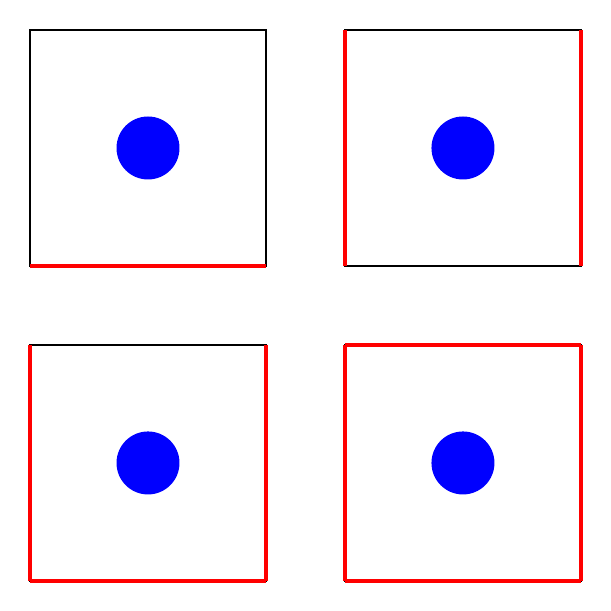
\begin{tikzpicture}
			\foreach \i/\x/\y in {1/0/4, 2/4/4, 3/0/0, 4/4/0} {

			\draw[thick] (\x,\y) rectangle ++(3,3);

			\ifnum\i=1 \draw[red, ultra thick] (\x,\y) -- ++(3,0); % bottom
			\fi \ifnum\i=2 \draw[red, ultra thick] (\x,\y) -- ++(0,3); % left
			\draw[red, ultra thick] (\x+3,\y) -- ++(0,3); % right
			\fi \ifnum\i=3 \draw[red, ultra thick] (\x,\y) -- ++(3,0); % bottom
			\draw[red, ultra thick] (\x,\y) -- ++(0,3); % left
			\draw[red, ultra thick] (\x+3,\y) -- ++(0,3); % right
			\fi \ifnum\i=4 \draw[red, ultra thick] (\x,\y) -- ++(3,0); % bottom
			\draw[red, ultra thick] (\x,\y+3) -- ++(3,0); % top
			\draw[red, ultra thick] (\x,\y) -- ++(0,3); % left
			\draw[red, ultra thick] (\x+3,\y) -- ++(0,3); % right
			\fi

			\fill[blue] (\x+1.5,\y+1.5) circle (0.4); }
		\end{tikzpicture}
	\end{center}
	Let all the flooded dots be contained in the circular blue region. Since the ``flood''
	increases in diameter upwards by $2$, Vulcan can build an arbitrarily large wall
	to the south at an arbitrary distance south. (since he places $3$ walls a turn).
	Now we build the side walls, each of which can grow at a rate of
	$\frac{3}{2} = 1.5 > 1$ walls per turn. Hence, these can be extended to an
	arbitrary distance, after which we build the final wall (as in the figure, highlighted
	in red). $\hfill \blacksquare$
	\newline
	\newline
	Note that this problem is a special case of \textbf{\textsf{USA Winter TST for
	IMO 2020 Problem 3}} where $\alpha = 3$. The problem is given below.
	\newline

	\textit{ Let $\alpha \geq 1$ be a real number. Hephaestus and Poseidon play a
	turn-based game on an infinite grid of unit squares. Before the game starts,
	Poseidon chooses a finite number of cells to be flooded. Hephaestus is building
	a levee, which is a subset of unit edges of the grid (called walls) forming a
	connected, non-self-intersecting path or loop*. The game then begins with Hephaestus
	moving first. On each of Hephaestus’s turns, he adds one or more walls to the levee,
	as long as the total length of the levee is at most $\alpha n$ after his $n$th
	turn. On each of Poseidon’s turns, every cell which is adjacent to an already flooded
	cell and with no wall between them becomes flooded as well. Hephaestus wins if
	the levee forms a closed loop such that all flooded cells are contained in the
	interior of the loop — hence stopping the flood and saving the world. For which
	$\alpha$ can Hephaestus guarantee victory in a finite number of turns no matter
	how Poseidon chooses the initial cells to flood?
	\newline
	*More formally, there must exist lattice points
	$\mbox{\footnotesize $A_{0}, A_{1}, \dotsc, A_{k}$}$, pairwise distinct except
	possibly $\mbox{\footnotesize $A_{0} = A_{k}$}$, such that the set of walls is
	exactly
	$\mbox{\footnotesize $\{A_{0}A_{1}, A_{1}A_{2}, \dotsc , A_{k-1}A_{k}\}$}$. Once
	a wall is built it cannot be destroyed; in particular, if the levee is a closed
	loop (i.e. $\mbox{\footnotesize $A_{0} = A_{k}$}$) then Hephaestus cannot add
	more walls. Since each wall has length $\mbox{\footnotesize $1$}$, the length
	of the levee is $\mbox{\footnotesize $k$}$. }
	\newline
	The answer ends up being $\alpha > 2.$ ~\\

	\begin{tcolorbox}
		[colback=white!5!white,colframe=purple!75!white,title=\textsf{Problem 2: (APMO
		2015)}, opacityback=1] Let $\mathbb{S}= \{2, 3, 4, \ldots\}$ denote the set of
		integers that are greater than or equal to $2$. Does there exist a function
		$f : \mathbb{S}\to \mathbb{S}$ such that
		\[
			f (a)f (b) = f (a^{2} b^{2} )\text{ for all }a, b \in S\text{ with }a \ne b
			?
		\]
	\end{tcolorbox}
	\hfill \emph{Angelo Di Pasquale, Australia}
	\subsection*{Solution:}
	We prove that there are no such functions.
	\newline
	\textbf{\textsf{Claim:}} If there exists $f \colon \mathbb{S}\to \mathbb{S}$ satisfying
	the given condition, then $\forall$ $x,y \in \mathbb{S}$
	\[
		\frac{f(x^{2})}{x} = \frac{f(y^{2})}{y}
	\]
	\textbf{\textsf{Proof:}} Consider distinct elements $p,q,r \in \mathbb{S}$ and
	WLOG let $p>q>r$. Then
	\[
		f(p^{4}q^{4}r^{4}) = f(p^{2}r^{2})f(q^{2}) = f(p)f(r)f(q^{2}) \text{ or }f(p^{4}
		q^{4}r^{4})= f(q^{2}r^{2})f(p^{2}) = f(q)f(r)f(p^{2})
	\]
	\[
		\implies f(p)f(r)f(q^{2})= f(q)f(r)f(p^{2}) \implies \frac{f(p^{2})}{p} = \frac{f(q^{2})}{q}
		. \quad \quad \quad \blacksquare
	\]
	Again, FTSOC, assume that $f$ exists. Now, clearly, there is $k \in \mathbb{Q}^{+}$
	such that $f(x) = kf(x^{2})$, $x \in \mathbb{S}$. Then
	\[
		f(a)f(b) = \frac{f(ab)}{k}\text{ from the functional equation.}
	\]
	Using the functional equation, we get
	\[
		f(a)f(a^{2}) = f(a^{6}) = f(a)f(a^{5}) \cdot k = f(a) f(a^{4}) f(a) \cdot k^{2}
		=f(a)f(a)\frac{f(a^{2})}{k} k^{2} =f(a)f(a)f(a^{2})k
	\]
	\[
		\implies f(x) = \frac{1}{k} \ \forall \ x\in \mathbb{S}\implies \frac{1}{k^{2}}
		= \frac{1}{k} \ (\because f(a)f(b) = f(a^{2}b^{2})) \ \implies k=1 \quad \Rightarrow
		\Leftarrow \quad \because 1 \not \in \mathbb{S}. \quad \blacksquare
	\]
	~\\
	\begin{tcolorbox}
		[colback=white!5!white,colframe=purple!75!white,title=\textsf{Problem 3: (EGMO
		2013)}, opacityback=1] Determine all integers $m$ for which the $m \times m$
		square can be dissected into five rectangles, the side lengths of which are
		the integers $1,2,3,\ldots,10$ in some order.
	\end{tcolorbox}
	\hfill \emph{Matti Lehtinen (Finland)}
	\subsection*{Solution:}
	\textbf{\textsf{Claim:}} $11 \leq m \leq 13$.
	\newline
	\textbf{\textsf{Proof:}} By rearrangement inequality, the maximum area of the
	rectangles is $10 \cdot 9+8 \cdot 7 + \dots 2 \cdot 1 = 90+56+30+12+2 = 190$
	and the minimum area is $10 \cdot 1 + 9 \cdot 2 + \dots + 5\cdot 6 = 110$. Then
	the area of the square which equals $m^{2}$ lies between $110$ and $190$ and hence
	$m$ lies between \texttt{ceil}$(\sqrt{110}) = 11$ and \texttt{floor}$(\sqrt{190}
	) = 13$. $\hfill \blacksquare$ ~\\ ~\\ \textbf{\textsf{Claim:}} $m=11,13$ form
	\emph{tileable} squares.
	\newline
	\textbf{\textsf{Proof:}} Consider the given tilings ($11 \times 11$ followed by
	$13 \times 13$).
	\newline
	\begin{center}
		\begin{asy}
			size(5cm);

            real s = 1;

            string[] cols =
			{"A","B","C","D","E","F","G","H","I","J","K"};

            pair square(string col, int row) { int x = search(cols, col); int y = row - 1; return (x*s, y*s); }

            void
			fillRect(string c1, int r1, string c2, int r2, pen fillColor) { int x1 = search(cols, c1); int x2 = search(cols, c2); 
                int y1 = r1 - 1; int y2 = r2 - 1; pair ll = (x1*s, y1*s); pair ur = ((x2+1)*s, (y2+1)*s); 
                fill(ll -- (ur.x,ll.y) -- ur -- (ll.x,ur.y) -- cycle, fillColor); 
                draw(ll -- (ur.x,ll.y) -- ur -- (ll.x,ur.y) -- cycle, black+1bp); }

            fillRect("A", 1, "C", 9, lightblue); 
			fillRect("A",10, "J",11, lightred); 
            fillRect("D",6, "J", 9, lightgreen); 
            fillRect("D", 1, "K", 5, yellow);
			fillRect("K", 6, "K", 11, orange); 
            for (int i = 0; i <= 11; ++i)
			{ draw((i*s, 0) -- (i*s, 11*s), black); draw((0, i*s) -- (11*s, i*s), black); }
		\end{asy}
	\end{center}
	~\\
	\begin{center}
		\begin{asy}
            size(6cm);
            
            int n = 13;
            real s = 1;
            string[] cols = {"A","B","C","D","E","F","G","H","I","J","K","L","M"};
            
            // Helper function to get column index from label
            int colIndex(string c) {
              return search(cols, c);
            }
            
            // Fill a rectangular region from (c1, r1) to (c2, r2) with color
            void fillRect(string c1, int r1, string c2, int r2, pen color) {
              int x1 = colIndex(c1), x2 = colIndex(c2);
              int y1 = r1 - 1, y2 = r2 - 1;
              int xmin = min(x1, x2), xmax = max(x1, x2);
              int ymin = min(y1, y2), ymax = max(y1, y2);
              
              for (int x = xmin; x <= xmax; ++x) {
                for (int y = ymin; y <= ymax; ++y) {
                  pair sq1 = (x, y)*s;
                  pair sq2 = (x+1, y+1)*s;
                  fill(box(sq1, sq2), color);
                }
              }
            
              draw((xmin*s, ymin*s)--((xmax+1)*s, ymin*s)--((xmax+1)*s, (ymax+1)*s)--(xmin*s, (ymax+1)*s)--cycle, black+1bp);
            }
            
            // Fill rectangles
            fillRect("A", 13, "J", 8, lightblue);
            fillRect("A", 7, "I", 1, lightred); 
            fillRect("K",13, "M", 6, lightgreen); 
            fillRect("J", 5, "M", 1, yellow); 
            fillRect("J", 6, "J", 7, orange);
            
            // Draw grid lines
            for (int i = 0; i <= n; ++i) {
              draw((i*s, 0) -- (i*s, n*s), black);
              draw((0, i*s) -- (n*s, i*s), black);
            }
            
		\end{asy}
	\end{center}
	~\\ \textbf{\textsf{Claim:}} $m=12$ (a $12 \times 12$ square) is not \emph{tileable}.
	\newline
	\textbf{\textsf{Proof:}}
	\begin{center}
		\begin{asy}
			size(160); pen thickBlack = black + 1.2bp;

			draw((0,0)--(1,0)--(1,1)--(0,1)--cycle, thickBlack);

            draw((0.3,0)--(0.3,0.6), thickBlack); draw((0,0.6)--(0.6,0.6),
			thickBlack); draw((0.6,0.6)--(0.6,1), thickBlack); draw((0.6,0.3)--(1,0.3),
			thickBlack); draw((0.6,0.6)--(0.6,0.3), thickBlack); draw((0.3,0.3)--(0.6,0.3),
			thickBlack);

			dot((0.3,0), black); dot((0.3,0.6), black); dot((0,0.6), black); dot((0.6,0.6),
			black); dot((0.6,1), black); dot((0.6,0.3), black); dot((1,0.3), black); dot((0.3,0.3),
			black);
		\end{asy}
	\end{center}
	If there exists such a tiling, then it must be similar to the diagram, with a rectangle
	in the center that does not touch the sides of the main $12 \times 12$ square.
	This can be seen from the fact that there are at least two rectangles of
	distinct dimensions on each side of the $12 \times 12$ square, since $12 > 10$.
	Label the rectangle covering the top left corner of the square ``$ABCD$''
	starting from the top left. Then $C$ is an \emph{opposite point}. Similarly,
	define the other \emph{opposite points}. None of the \emph{opposite points} can
	coincide, since then we will invariably get rectangles of equal lengths. Hence,
	the \emph{opposite points} form a rectangle, and since there are exactly $5$
	rectangles, if a tiling is possible, then it must be of the form seen above. (See
	the $11 \times 11$ and $13 \times 13$ tilings for further examples).
	\newline
	Since $12-1=11>10$ and $12-6=6$, the rectangles covering the corners cannot have
	a side of $1,6$. Hence the middle rectangle (formed by the \emph{opposite
	points}) is of dimensions $1\times 6$. Then we need to divide
	$\{2,3,4,5,7,8,9,10 \}$ into $2-$tuples $(a,b)$ such that the $a-b = \pm 1,\pm6$.
	Then $7$ pairs with $8$ since none of $13, 1, 6$ are available and $4$ pairs
	with $5$, since none of $6, -1, 11$ are available. Now $\{2,3,9,10\}$ cannot
	be divided into $2-$tuples $(a,b)$ with $a-b = \pm 6$, so no tiling is
	possible and we are done. $\hfill \blacksquare$ ~\\
	\begin{tcolorbox}
		[colback=white!5!white,colframe=purple!75!white,title=\textsf{Problem 4: (Balkan
		MO 2022)}, opacityback=1] Let $a, b$ and $n$ be positive integers with $a>b$
		such that all of the following hold:
		\newline

		\textbf{(i.)} $a^{2021}$ divides $n$.
		\newline
		\textbf{(ii.)} $b^{2021}$ divides $n$.
		\newline
		\textbf{(iii.)} 2022 divides $a-b$.
		\newline
		\newline
		Prove that there is a subset $T$ of the set of positive divisors of the number
		$n$ such that the sum of the elements of $T$ is divisible by 2022 but not divisible
		by $2022^{2}$.
	\end{tcolorbox}
	\hfill \emph{Silouanos Brazitikos, Greece}
	\subsection*{Solution:}
	We write $a \mid b$ to mean $a$ divides $b$.
	\newline
	Let $d=$gcd($a,b$) and hence let $a=dp$ and $b=dq$, where $p,q$ are co-prime.
        Then $d^{2021}p^{2021}q^{2021} \mid n$ and $2022 \mid d(p-q)$. \newline \newline
        Let $f_{2022}(x)$ denote the highest power of $2022$ that divides $x$; i.e, $2022^{f_{2022}(x)} \mid x$ but 
        $2022^{f_{2022}(x) + 1} \nmid x$. We split into $3$ cases: \newline \newline
        \textbf{Case 1:} $f_{2022}(d) \ge 2$. \newline
        \textbf{Solution:} Take $T = \{1011^2, 1011 \}$. $\hfill \blacksquare$ \newline \newline
        \textbf{Case 2:} $f_{2022}(d) = 1$. \newline
        \textbf{Solution:} Take $T = \{d \}$. $\hfill \blacksquare$ \newline \newline
        \textbf{Case 3:} $f_{2022}(d) = 0$. \newline
        \textbf{Solution:} 
        \[ \text{We claim that } T=\{p^kq^{2021-k} \colon k \in \{0,1, 2, \dots, 2021 \} \} \text{ or } S=\frac{p^{2022}-q^{2022}}{p-q} = \sum_{k=0}^{2021} p^kq^{2021-k} \text{ is the required sum.}\]
        \textbf{Proof:} \newline 
        Firstly, $\forall \ x \in T$, $x \mid 2022 \because \ p,q$ are co-prime and $p^{2021}q^{2021} \mid n$. \newline
        Secondly, note that $f_{2022}(d) = 0 \implies p \equiv q \pmod{2022}$. Then: \[S=\sum_{k=0}^{2021} p^kq^{2021-k} \equiv \sum_{k=0}^{2021}p^{2021} \equiv0 \pmod{2022}.\]
        Also, $2022 = 2 \cdot 3 \cdot 337$. As usual, denote by $v_p(n)$ the highest power of $p$ that divides $n$.
        Clearly, all $3$ of $2,3,337$ cannot divide $p$, because then $2022 \mid p \implies 2022 \mid q \ (\because p \equiv q \pmod{2022})$ which is a contradiction.
        Hence, one of $2,3,337$ does not divide $p$. WLOG, let it be $337$. Then:
         \[p \equiv q \pmod{2022} \implies p\equiv q \pmod{337} \implies 337 \nmid p \iff 337 \nmid q.\]
         Hence, $337 \nmid q$.  Now we can apply \textbf{Lifting The Exponent Lemma}:  \[ v_{337}\left(\frac{p^{2022} - q^{2022}}{p-q} \right) = v_{337}(p-q)+v_{337}(n) - v_{337}(p-q) \]
         Since $n=2022$ and $v_{337}(2022) = 1$, $v_{337}(S) = 1 \implies 337^2 \nmid S \implies 2022^2 \nmid S$. $\hfill \blacksquare$ \newline \newline
         \textbf{Note:} If the prime picked is $2$; then $3 \cdot 337 \mid p$, or we could have picked any of $3, 337$ and be done as before.
         Then $1011 \mid p \implies 1011^{2021} \mid n \implies T= \{1011, 1011^2\}$ suffices. $\hfill \blacksquare$
         
\end{document}
